
\documentclass[conference]{IEEEtran}
\IEEEoverridecommandlockouts
% The preceding line is only needed to identify funding in the first footnote. If that is unneeded, please comment it out.
\usepackage{cite}
\usepackage{amsmath,amssymb,amsfonts}
\usepackage{algorithmic}
\usepackage{graphicx}
\usepackage{textcomp}
\usepackage{xcolor}
\usepackage{tikz}
\usetikzlibrary{positioning,fit,arrows.meta,shapes.geometric,calc}


\def\BibTeX{{\rm B\kern-.05em{\sc i\kern-.025em b}\kern-.08em
    T\kern-.1667em\lower.7ex\hbox{E}\kern-.125emX}}
\begin{document}

\title{A model for object detection and semantic segmentation applicable to the CamVid dataset\\
{\footnotesize \textsuperscript{*}Based on Yolo and Deeplab architectures - COMP0248}
}

\author{\IEEEauthorblockN{Jiaqi Yao}}

\maketitle

\begin{abstract}

    %  这篇论文介绍了一种混合模型,该模型综合了 Yolo 系列和 DeeplabV3 架构的优势,利用 CamVid 数据集同时进行物体检测和语义分割。具体来说,该研究通过开发定制的数据增强策略和焦点损失优化,解决了类不平衡和数据集规模有限带来的重大挑战。由此产生的模型实现了合理的分割准确度(mIoU 约为 0.5)和有限的对象检测(map@0.5 约为 0.25)

 This coursework paper presents a hybrid model for simultaneous object detection and semantic segmentation using the CamVid dataset, integrating the strengths of Yolo series and DeeplabV3 architectures. Specifically, the study addresses the significant challenges posed by class imbalance and limited dataset size by developing customized data augmentation strategies and focal loss optimization. The resulting model achieves reasonable segmentation accuracy (mIoU around 0.5) and limited object detction(map@0.5 around 0.25).

\end{abstract}

\begin{IEEEkeywords}
object detection, semantic segmentation, Yolo, Deeplabv3, CamVid dataset
\end{IEEEkeywords}

\section{Introduction}
% 计算机视觉在近年来取得了显著的进展,然而机器仍然难以像人类一样准确理解城市环境。因此,在本课程作业中,我们尝试使机器能够准确识别和分割街景中的对象,使用CamVid(Cambridge-driving Video)数据集。

% 具体来说,这涉及到机器具有识别道路、建筑物、行人、车辆和其他元素的能力,就像人类通过步行或驾驶在城市中导航一样。

% 为了解决这些挑战,我们将根据YoloV3和Deeplabv3架构的思想重新编程和构建模型,分别是目标检测和语义分割。为了防止过拟合,我们将简化和修改大部分架构,以便我们可以在小数据集(如CamVid数据集)上训练模型,并评估其在mAP、IoU和其他指标方面的性能。我们还将探索各种处理类别不平衡的技术,并分析它们对模型性能的影响。

% 计算机视觉技术已经取得了长足的进步,但要准确理解城市场景仍然具有挑战性,尤其是在处理 CamVid 这样的小型不平衡数据集时。本文的重点是通过调整 YOLOv3 和 DeeplabV3 架构,增强街道场景的物体检测和语义分割能力。具体来说,我们通过有针对性的模型修改和专门的训练技术,解决了五种常见类别(汽车、行人、自行车、摩托车和公共汽车)的类别不平衡问题,最终通过 mAP 和 IoU 等指标评估了性能。
Computer vision has made significant progress in recent years; however, machines still struggle to comprehend urban environments with the same level of understanding as humans. So, in this coursework, we try to enable machines to accurately identify and segment objects in street scenes using the CamVid (Cambridge-driving Video) dataset.\cite{b3}
 
Specifily, this involves the robots with the ability to recognize roads, buildings, pedestrians, vehicles, and other elements in their surroundings—like a human navigating a city by walking or driving.

To address these challenges, we reprogram and build the model with the help of ideas from the Yolo and Deeplabv3 architectures, object detection and semantic segmentation, respectively. To prevent overfitting compared to the original model, we will streamline and modify most of the architectures so that we can train the model on small datasets such as the CamVid dataset and evaluate its performance in terms of mAP, IoU, and other metrics. We will also explore various techniques for dealing with class imbalance and analyze their impact on model performance.
\section{Dataset}
% 5 class distribution, preprocessing steps, data visualization etc.
\subsection{CamVid Dataset Overview}
% CamVid 数据集是相比其他数据集(如COCO,Cityscapes))是较小的数据集。其中包含了街景图像和对应的像素级标注,可用于语义分割任务。数据集中包含32个类别,但我们只关注其中的5个类别:汽车、行人、自行车、摩托车和公共汽车并将其他设为背景。 此外,我们还根据对应的像素级标注,生成对应的适用于目标检测的框标注,以便进行目标检测任务。
The CamVid dataset is a relatively small dataset compared to others like COCO and Cityscapes. It consists of street scene images and corresponding pixel-level annotations for semantic segmentation tasks. The dataset contains 32 classes, but we focus only on five classes: cars, pedestrians, bicycles, motorcycles, and buses, with the rest labeled as background. Additionally, we generate bounding box annotations suitable for object detection tasks based on the corresponding pixel-level annotations.

\subsection{Data Preprocessing}
%  对于数据的预处理, camvid提供的标签是灰度的掩码图像,是可以直接被用于语义分割的训练。 我们需要做的就是增加一个过滤器,将原有的标签图像进行过滤使其只保留5个我们关系的类别,并将其转换为像素值为0-5的标签图像。(0表示背景) 。 

% 具体的操作为: 首先读取包含元数据映射关系的csv文件 之后对其使用filter_classes 函数,将标签过滤,只保留我们需要的5个类别并将其他设为0(背景)。之后创建一个和原图像一样大小的全0矩阵,然后将过滤后的标签放入对应的位置。

For the data preprocessing, the labels provided by CamVid are grayscale mask images that can be directly used for semantic segmentation training. We need to add a filter to the original label images to retain only the five classes we are interested in and convert them into label images with pixel values of 0-5 (0 represents background).

The details are as follows: first, read the CSV file containing the metadata mapping, then use the \textbf{filter\_classes} function to filter the labels, keeping only the five classes we need and setting the rest to 0 (background). Then create a full zero matrix the same size as the original image and place the filtered labels in the corresponding positions.

% 此外,对于物品检测框的构建,首先过滤掉面积过小的像素,然后根据连通域分析的方法筛选出需要绘制目标检测框的区域,再根据每个单独区域建立物品检测框,即以像素区的上下左右四个顶点绘制检测框,之后按照cxcywh的格式转换为yolo的物品检测标签。注意这里的cxcy是对于单元格内的归一化,wh是相对于整个图像的归一化。

In addition, for the construction of object detection boxes, first filter out pixels with small areas, then use the method of connected domain analysis to select the areas that need to draw object detection boxes, and then establish object detection boxes for each separate area, that is, draw detection boxes with the upper, lower, left, and right four vertices of the pixel area, and then convert them to Yolo object detection labels in the format of cxcywh. Note that cxcy here is normalized within the cell, and wh is normalized relative to the entire image.


% An example is shown as figure \ref{fig:format}.
% % 例子如下所示:
% \begin{figure}[htbp]
%     \centerline{\includegraphics[width=0.4\textwidth]{fig/yolo_format.jpg}}
%     \caption{Example of Yolo Format}
%     \label{fig:format}
% \end{figure}

% 其中每个yolo标签的形状为(Sx,Sy,C+B*5),其中Sx和Sy是图像块的维度,C是类别数,B是每个网格单元的边界框数。

The shape of each yolo label is (Sx, Sy, C+B*5), where Sx and Sy are the dimensions of the image block, C is the number of classes, and B is the number of bounding boxes per grid cell.


% 此外,关于数据类型不平衡的特点,我们构建了一个数据增强器,当检测到加载的图像里面包含少数类的图像时进行增强(摩托车和公交车)。增强方式使用了随机翻转、旋转、和颜色抖动等方法。
Moreover, to address the issue of class imbalance, we built a data augmenter to enhance images containing minority classes (motorcycles and buses) when detected. The augmentation methods include random flipping, rotation, and color jittering.

\subsection{Data Visualization and Analysis}

% 经过预处理的数据示例如下所示
The preprocessed data is shown as follows in figure \ref{fig:data}.

\begin{figure}[htbp]
    \centerline{\includegraphics[width=0.5\textwidth]{fig/data.png}}
    \caption{Preprocessed Data Example}
    \label{fig:data}
\end{figure}


\section{Methodology}
% Model architecture, training details, design choices
\subsection{Model Architecture}

% 在模型的构建上我们借助了DeeplabV3和Yolo的思想,并将两个模型融合起来。他们共同使用一个特征提取头(ResNet50),然后分别用于目标检测和语义分割任务。其中的语义分割部分,我们使用了DeeplabV3的骨干网络,即ASPP(空间金字塔池化模块),并在其基础上进行了改进了输出头,以适应CamVid数据集的特点。目标检测部分,将yolo的输出头进行简化并且拼接到特征提取头的后面。这里的yolo输出头使用v2v3的架构使用卷积层代替了v1的全连接层,以提高模型的性能。

In the construction of the model, we borrowed ideas from DeeplabV3 and Yolo and combined the two models. They share a common feature extraction backbone (ResNet50) \cite{b0} and are then used for object detection and semantic segmentation tasks, respectively. For the semantic segmentation part, we used the DeeplabV3+ backbone network, namely ASPP (Atrous Spatial Pyramid Pooling) \cite{b2}, and improved the output head based on it to adapt to the characteristics of the CamVid dataset. For the object detection part, we simplified the output head of Yolo and concatenated it to the back of the feature extraction backbone. The Yolo output head here uses the architecture of v2\cite{b6}v3\cite{b1}, replacing the fully connected layers of v1 \cite{b7} with convolutional layers to improve the performance of the model.

% 模型架构如下图3所示

The model architecture is shown in figure \ref{fig:architecture}.

\begin{figure}[htbp]
    \centering
    \scalebox{0.6}{ % 将整个图形缩小至0.8倍
    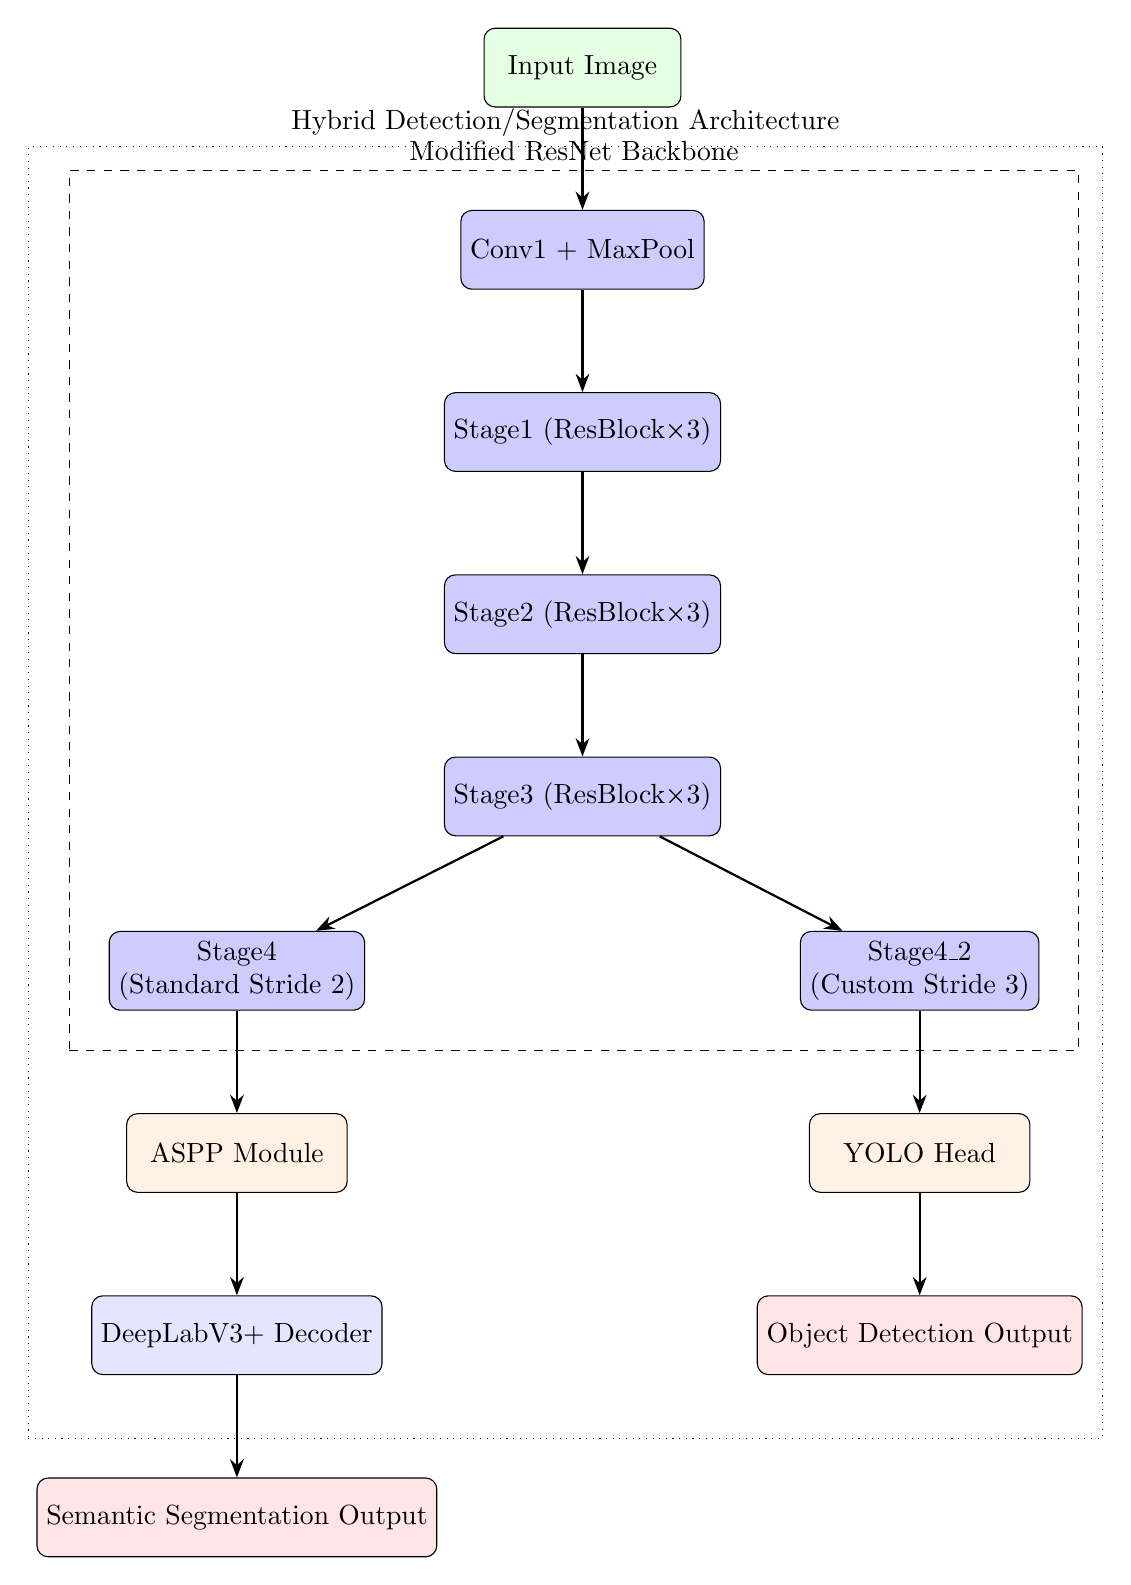
\begin{tikzpicture}[
        block/.style={draw, fill=blue!10, rounded corners, minimum width=2.8cm, minimum height=1cm, align=center},
        arrow/.style={-Stealth, thick},
        input/.style={draw, fill=green!10, rounded corners, minimum width=2.5cm, minimum height=1cm, align=center},
        output/.style={draw, fill=red!10, rounded corners, minimum width=2.5cm, minimum height=1cm, align=center},
        module/.style={draw, fill=orange!10, rounded corners, minimum width=2.8cm, minimum height=1cm, align=center},
        feature/.style={draw, fill=yellow!10, rounded corners, minimum width=2.8cm, minimum height=1cm, align=center},
        backbone/.style={draw, fill=blue!20, rounded corners, minimum width=2.8cm, minimum height=1cm, align=center},
        node distance=1.3cm
    ]
    
    % 输入节点
    \node[input] (input) {Input Image};
    
    % 骨干网络部分
    \node[backbone, below=of input] (conv1) {Conv1 + MaxPool};
    \node[backbone, below=of conv1] (stage1) {Stage1 (ResBlock×3)};
    \node[backbone, below=of stage1] (stage2) {Stage2 (ResBlock×3)};
    \node[backbone, below=of stage2] (stage3) {Stage3 (ResBlock×3)};
    
    % 分支路径
    \node[backbone, below left=1.2cm and 1.0cm of stage3] (stage4) {Stage4\\(Standard Stride 2)};
    \node[backbone, below right=1.2cm and 1.0cm of stage3] (stage4_2) {Stage4\_2\\(Custom Stride 3)};
    
    % 特征提取后的路径
    \node[module, below=of stage4] (aspp) {ASPP Module};
    \node[block, below=of aspp] (decoder) {DeepLabV3+ Decoder};
    \node[output, below=of decoder] (segout) {Semantic Segmentation Output};
    
    \node[module, below=of stage4_2] (yolohead) {YOLO Head};
    \node[output, below=of yolohead] (detout) {Object Detection Output};
    
    % 连接箭头
    \draw[arrow] (input) -- (conv1);
    \draw[arrow] (conv1) -- (stage1);
    \draw[arrow] (stage1) -- (stage2);
    \draw[arrow] (stage2) -- (stage3);
    \draw[arrow] (stage3) -- (stage4);
    \draw[arrow] (stage3) -- (stage4_2);
    \draw[arrow] (stage4) -- (aspp);
    \draw[arrow] (aspp) -- (decoder);
    \draw[arrow] (decoder) -- (segout);
    \draw[arrow] (stage4_2) -- (yolohead);
    \draw[arrow] (yolohead) -- (detout);
    
    % 标注骨干网络框架
    \node[draw, dashed, fit=(conv1)(stage1)(stage2)(stage3)(stage4)(stage4_2), inner sep=0.5cm, label=above:Modified ResNet Backbone] {};
    
    % 标注整体架构
    \node[draw, dotted, fit=(conv1)(stage1)(stage2)(stage3)(stage4)(stage4_2)(aspp)(decoder)(yolohead), inner sep=0.8cm, label=above:Hybrid Detection/Segmentation Architecture] {};
    
    \end{tikzpicture}
    } % 缩放结束
    \caption{Model Architecture}
    \label{fig:architecture}
\end{figure}

% 在这里Resnet50的细节架构见论文[1],我们不再赘述。这里值得注意的是为了对其yolo输出头的格式,我们对于resnet50的最后一个残差块进行了并行处理,额外分了一条支路使用步长为3的卷积连接yolo的输出头。根据计算,前三层之后的特征图大小为960/16=60,720/16=45。经过第四层卷积后,特征图大小为60/3=20,45/3=15。

The detailed architecture of ResNet50 can be found in the paper, and we will not repeat it here. It is worth noting that for the format of the Yolo output head, we parallelly processed the last residual block of ResNet50, and an additional branch was created to connect the Yolo output head with a convolutional layer with a stride of 3.

% 在这主要介绍ASPP模块和Yolo的输出头。aspp架构如图所示:
Here we mainly introduce the ASPP module and the output head of Yolo. The ASPP architecture is as shown in figure \ref{fig:aspp}.

\begin{figure}[htbp]
    \centering
    \centerline{\includegraphics[width=0.5\textwidth]{fig/aspp.png}}
    \caption{ASPP Module Architecture}
    \label{fig:aspp}
\end{figure}

% ASPP模块是DeepLabv3的核心组件,它通过多尺度的空洞卷积来捕获不同尺度的上下文信息。在我们的模型中,我们使用了四个不同尺度的空洞卷积,分别是1、12、24、36,然后将它们拼接在一起,通过一个1x1的卷积层来融合这些信息。具体架构如下所示:

The ASPP module is the core component of DeepLabV3, which captures context information at different scales through multi-scale atrous convolutions. In our model, we use four different scales of atrous convolutions, namely 1, 12, 24, and 36, and then concatenate them together to fuse this information through a 1x1 convolutional layer. The specific architecture is as shown in figure \ref{fig:aspp}.

% YOLO 的输出头将会直接连接在ResNet50的输出上,他包含了全连接层和激活函数,最终输出的形状是(Sx,Sy,C+5B),其中Sx和Sy是图像块的维度,C是类别数,B是每个网格单元的边界框数。

The output head of YOLO will be directly connected to the output of ResNet50, which includes fully connected layers and activation functions, and the final output shape is (Sx, Sy, C+5B), where Sx and Sy are the dimensions of the image block, C is the number of classes, and B is the number of bounding boxes per grid cell. 

% 因为在默认的yolov1中, Sx=Sy=7,C=20,B=2。 在yolov3中,三个输出尺度分别是52x52, 26x26, 13x13,这里为了保持和resnet的输出一致,我们设置Sx=20,Sy=15,C=5,B=1。具体架构如下所示:

Because in the default YOLOv1, Sx=Sy=7, C=20, B=2. In YOLOv3, the three output scales are 52x52, 26x26, 13x13. Here, to keep it consistent with the output of ResNet, we set Sx=20, Sy=15, C=5, B=1. The specific architecture is as shown in figure \ref{fig:yolo}.


\begin{figure}
\centering
\scalebox{0.6}{
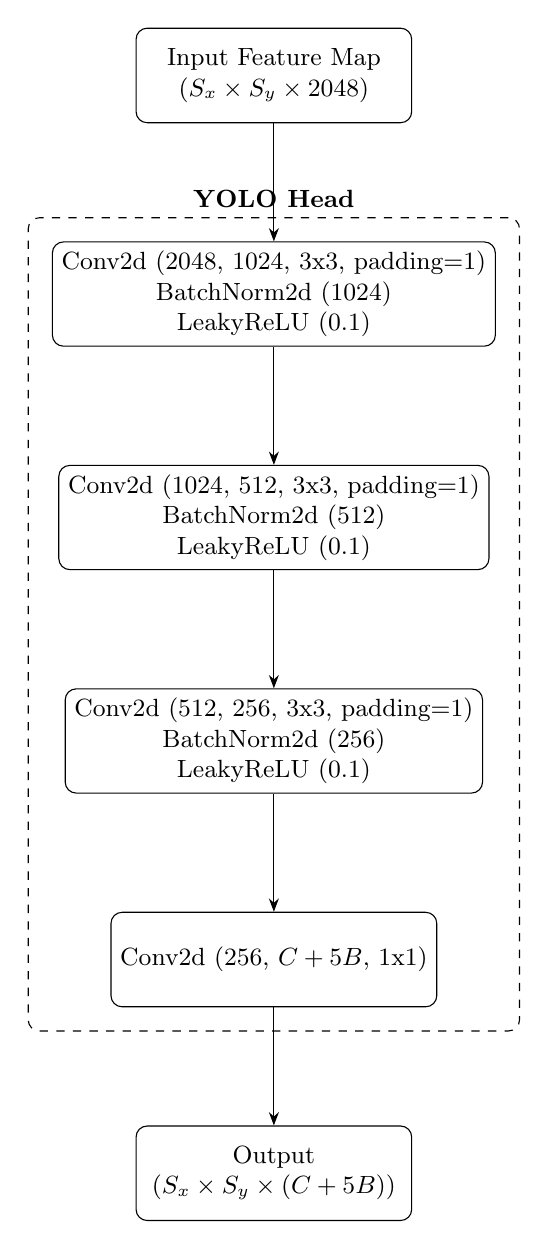
\begin{tikzpicture}[
    font=\small, 
    node distance=1.5cm, 
    >=Stealth, 
    block/.style={draw, rectangle, rounded corners, align=center, minimum width=3.5cm, minimum height=1.2cm},
    bigblock/.style={draw, dashed, rounded corners, inner sep=0.3cm}
]

% 输入特征图
\node[block] (input) {Input Feature Map\\\((S_x \times S_y \times 2048)\)};

% Conv1
\node[block, below=1.5cm of input] (conv1) {Conv2d (2048, 1024, 3x3, padding=1)\\BatchNorm2d (1024)\\LeakyReLU (0.1)};

% Conv2
\node[block, below=1.5cm of conv1] (conv2) {Conv2d (1024, 512, 3x3, padding=1)\\BatchNorm2d (512)\\LeakyReLU (0.1)};

% Conv3
\node[block, below=1.5cm of conv2] (conv3) {Conv2d (512, 256, 3x3, padding=1)\\BatchNorm2d (256)\\LeakyReLU (0.1)};

% 输出层
\node[block, below=1.5cm of conv3] (conv_out) {Conv2d (256, \(C + 5B\), 1x1)};

% 输出
\node[block, below=1.5cm of conv_out] (output) {Output\\\((S_x \times S_y \times (C + 5B))\)};

% 连接箭头
\draw[->] (input.south) -- (conv1.north);
\draw[->] (conv1.south) -- (conv2.north);
\draw[->] (conv2.south) -- (conv3.north);
\draw[->] (conv3.south) -- (conv_out.north);
\draw[->] (conv_out.south) -- (output.north);

% 用虚线框标注 YOLO Head
\node[bigblock, fit=(conv1)(conv2)(conv3)(conv_out), label=above:\textbf{YOLO Head}] (yolo_head) {};

\end{tikzpicture}}
\caption{Yolo Output Head Architecture}
\label{fig:yolo}
\end{figure}


\subsection{Design Choices and Innovations}
% This subsection introduces the key decisions and specific optimizations made in the model design to adapt to the CamVid dataset.

% 在模型设计中,我们做出了一些关键决策和特定优化,以适应CamVid数据集。

% 从特征提取的角度来看,我们选择了公认的具有优秀表现的特征提取网络ResNet50作为我们的骨干网络,因为它在深度和计算效率之间有着出色的平衡。ResNet的创新残差连接通过提供梯度快捷方式使更深的网络能够有效训练,从而缓解了梯度消失问题。这种架构通过其分阶段设计优秀地提取了分层特征——早期层捕获低级特征如边缘和纹理,而更深层次则识别复杂的物体模式。

% 我们的创新点事通过在最后的卷积阶段实现了一个双分支方法,从而修改了标准的ResNet50结构。这种修改创建了两个并行的特征提取路径:一个保持语义分割任务的原始步幅(保留空间分辨率),另一个使用自定义步幅3用于目标检测分支(降低维度但保留重要特征)。

In the model design, we made some key decisions and specific optimizations to adapt to the CamVid dataset.

From a feature extraction perspective, we selected the widely recognized feature extraction network ResNet50 as our backbone network due to its excellent balance between depth and computational efficiency. ResNet's innovative residual connections allow deeper networks to train effectively by providing gradient shortcuts, thus mitigating the vanishing gradient problem. This architecture excels at extracting hierarchical features through its staged design - early layers capture low-level features like edges and textures, while deeper layers recognize complex object patterns.

Our innovation is to implement a dual-branch approach in the final convolution stage, thus modifying the standard ResNet50 structure. This modification creates two parallel feature extraction paths: one maintains the original stride for the semantic segmentation task (preserving spatial resolution), while the other uses a custom stride of 3 for the object detection branch (reducing dimensionality but retaining important features).


% 对于语义分割来说,一个很重要的问题是如果按照典型的cnn模型进行连续的下采样和重复池化,不仅会导致最后特征图分辨率过低的问题,还会使得图中的大尺度和多尺度的物品被压缩进而丢失信息。在这我借用deepLabv3的思想,使用了ASPP模块来解决这个问题。ASPP模块通过多尺度的空洞卷积来捕获不同尺度的上下文信息,提高了模型的性能。此外我们还在ASPP模块的基础上进行了更新,使用空洞卷积来防止模型对大尺度物品丢失信息的情况。最后再使用deeplabv3+的输出头将输出形状设置为(CxHxW)的形式,用以代表每个像素的类别。


For semantic segmentation, a critical issue is that if the typical CNN model is used for continuous downsampling and repeated pooling, it will not only lead to the problem of too low resolution of the final feature map but also compress large-scale and multi-scale objects in the image, resulting in information loss. Here, I borrowed the idea of DeepLabV3 and used the ASPP module to solve this problem. The ASPP module captures context information at different scales through multi-scale atrous convolutions, improving the performance of the model. In addition, we also updated the ASPP module to use atrous convolutions to prevent the model from losing information about large-scale objects. Finally, we used the output head of DeeplabV3+ to set the output shape to (CxHxW) to represent the category of each pixel.

% 对于物品检测,我们参考了yolov1v2v3三个版本的思想,考虑到数据集的大小,担心过拟合的问题,只使用了一种尺度的输出网格(20*15),并且只使用了一个边界框。此外,考虑到后续版本的yolo输出头都使用了卷积层代替了全连接层,我们也使用了这种方法。这种方法可以减少参数数量,提高模型的性能。

For object detection, we referred to the ideas of YOLOv1, v2, and v3. Considering the size of the dataset and the risk of overfitting, we only used one scale of output grid (20*15) and only one bounding box. In addition, considering that the output head of later versions of YOLO all used convolutional layers instead of fully connected layers, we also used this method. This method can reduce the number of parameters and improve the performance of the model.

\subsection{Training Strategy}
% This subsection introduces the training process, loss function selection, optimizer settings, and other details.

% 在训练过程中的损失函数上,我们使用了交叉熵损失函数来计算deeplab语义分割的损失,使用均方差来计算yolo目标检测的损失(和yolov1一样的损失函数计算方法)。在优化器上,我们使用了Adam优化器,学习率为 1e-4,一共训练500个epoch。同时设置早停机制(在100epoch后触发),当验证集上的损失不再下降时,停止训练。记录训练数据和验证数据的损失,以便后续分析。

%同时为了提高训练速度,在合适的计算过程中我们开启了半精度计算(fp16)。

In the training process, we used the cross-entropy loss function to calculate the loss of Deeplab semantic segmentation and the mean square error to calculate the loss of Yolo object detection (the same loss calculation method as YOLOv1). For the optimizer, we used the Adam optimizer with a learning rate of 1e-4 and trained for a total of 500 epochs. We also set up an early stopping mechanism (triggered after 100 epochs) to stop training when the loss on the validation set no longer decreases. We recorded the loss of the training data and validation data for subsequent analysis.

To improve training speed, we enabled mixed precision computing (fp16) in appropriate calculations.

% 另一个值得注意的点是,在损失函数中我们启用了focalloss,这是一种针对类别不平衡问题的损失函数。我们分别对语义分割的损失和yolo的损失进行了focalloss的计算,以提高模型对少数类的识别能力。具体的实现细节见后文的类别不平衡章节。

Another point worth noting is that we enabled focal loss in the loss function, which is a loss function for class imbalance problems.\cite{b4} We calculated the focal loss for both the loss of semantic segmentation and the loss of Yolo to improve the model's ability to recognize minority classes. The specific implementation details are described in the following section on class imbalance.

% 语义分割和目标检测的损失函数加在一起为最终的损失函数。

The loss functions for semantic segmentation and object detection are added together to form the final loss function.

\section{Experimental Setup}
% hyperparameters, etc.
\subsection{Experimental Environment}
% This subsection describes the hardware and software environment used for the experiments.

%所有的训练都是在CS服务器上进行的,并且结果都是可以复现的。我们在数据加载中设置的批次大小是按照16G显存的gpu进行设置的,并且在合适的地方开启了半精度计算。

%相关的pytorch版本是2.6 cuda版本12.6, python版本应该是3.9以上都可以(3.8和最新的3.13在测试后也没问题)。 其中使用的外部库除了常用的numpy,json外还使用了opencv用作联通域分析。相关仓库的github连接将会附在报告后面。用到的库基本都是常用库。

All training was done on the CS server, and the results are reproducible. The batch size set in the data loading is based on the 16G GPU, and mixed precision computing is enabled in appropriate places.

The relevant PyTorch version is 2.6, CUDA version is 12.6, and the Python version should be 3.9 or above (3.8 is also fine, and the latest 3.13 has been tested without any problems). In addition to the commonly used libraries such as NumPy and JSON, we also used OpenCV for connected domain analysis. The GitHub link to the relevant repository will be attached at the end of the report. The libraries used are mostly common libraries.



\subsection{Hyperparameter Settings}
% This subsection lists in detail the hyperparameters used in the training process, such as learning rate, batch size, number of epochs, etc., and explains the reasons for these choices.

% 表1展示了我们训练过程中使用的关键超参数。
Table \ref{tab:hyperparams} presents the key hyperparameters used in our training process.

\begin{table}[htbp]
    \caption{Hyperparameter Settings}
    \label{tab:hyperparams}
    \centering
    \begin{tabular}{cc}
    \hline
    \textbf{Hyperparameter} & \textbf{Value} \\
    \hline
    Optimizer & Adam \\
    Initial learning rate & 1e-4 \\
    Learning rate schedule & Step decay \\
    Batch size & 16 \\
    The minimum epochs & 125 \\
    Early stopping patience & 10 \\
    Input image size & 960*720 \\
    Mixed precision & Enable \\
    \hline
    \end{tabular}
    \end{table}


% 对于语义分割头,我们采用交叉熵损失,并使用γ=2.0的focal loss改进版来应对类别不平衡。类别权重(α)按训练集的逆频率确定:背景(0.1)、汽车(0.8)、行人(0.6)、自行车(0.9)、摩托车(0.9)和公共汽车(0.9)。

% 对于目标检测头,我们使用均方误差损失,遵循YOLOv1方法,并将置信度阈值设为0.5进行非极大值抑制。批归一化层的动量设为0.9,以平衡训练稳定性和适应性。

% 批次大小为16在内存效率和收敛速度之间实现最佳折衷,较小批次导致训练不稳定,较大批次超出GPU内存。学习率衰减至关重要,因训练40个epoch后保持初始学习率会引发验证损失波动。

% 为防止在CamVid小数据集上过拟合,我们采用早停机制,耐心值设为15个epoch,并监测验证损失,使模型能持续学习但避免严重过拟合。

For the semantic segmentation head, we used cross-entropy loss and an improved version of focal loss with γ=2.0 to address class imbalance. The class weights (α) were determined based on the inverse frequency of the training set: background (0.1), car (0.8), pedestrian (0.6), bicycle (0.9), motorcycle (0.9), and bus (0.9).

For the object detection head, we used mean square error loss, following the YOLOv1 method, and set the confidence threshold to 0.5 for non-maximum suppression. The momentum of the batch normalization layer was set to 0.9 to balance training stability and adaptability.

A batch size of 16 achieved the best compromise between memory efficiency and convergence speed, with smaller batches leading to unstable training and larger batches exceeding GPU memory. Learning rate decay is crucial, as keeping the initial learning rate after 40 epochs will cause fluctuations in the validation loss.

To prevent overfitting on the small CamVid dataset, we used an early stopping mechanism with a patience value of 15 epochs and monitored the validation loss to allow the model to continue learning while avoiding severe overfitting.



\subsection{Evaluation Metrics}
% This subsection explains the metrics used to evaluate model performance, such as mAP, IoU, etc., and the calculation methods for these metrics.

% 在这里我们使用了两个主要的评估指标:miou和map。其中miou主要用于语义分割任务,map主要用于目标检测任务。在这里我们取概率为0.5的预测为有效预测。对于物品检测,因为包含两个概率分别是置信度和类别概率,我们使用了coco的评估方式。在这里使用当联合概率分布大于0.05时,我们认为是有效预测。(P_{obj} * P_{class} > 0.05)

Here we used two main evaluation metrics: mIoU and mAP. mIoU is mainly used for semantic segmentation tasks, while mAP is mainly used for object detection tasks. Here we considered predictions with a probability of 0.5 as valid predictions. For object detection, because it contains two probabilities, confidence and class probability, we used the COCO evaluation method.\cite{b5} Here we considered it a valid prediction when the joint probability distribution was greater than 0.05 ($P_{obj} * P_{class} > 0.05$).

% miou是交并比(IoU)的平均值,计算公式如下:

mIoU is the average of the Intersection over Union (IoU), calculated as follows:
\[IoU = \frac{TP}{TP + FP + FN}\]
\[mIoU = \frac{1}{N} \sum_{i=1}^{N} IoU_i\]

% map是平均精度(AP)的平均值,计算公式如下:

mAP is the average of the average precision (AP), calculated as follows:

\[AP = \frac{1}{N} \sum_{r \in \{0.0, 0.1, \ldots, 1.0\}} p(r)\]

\[mAP = \frac{1}{C} \sum_{c=1}^{C} AP_c\]

% 其中,TP表示真阳性,FP表示假阳性,FN表示假阴性,N表示类别数,C表示类别数。

Where TP is true positive, FP is false positive, FN is false negative, N is the number of classes, and C is the number of classes.

\section{Results}
% mAP/IoU scores, class-wise analysis, qualitative results

%训练过程中的损失和准确率如下图所示:

The loss and accuracy during training are shown in the figure \ref{fig:loss}.

\begin{figure}[htbp]
    \centerline{\includegraphics[width=0.5\textwidth]{matrials/training_results.png}}
    \caption{Training Loss and Accuracy}
    \label{fig:loss}
\end{figure}

% 损失收敛于0.25左右 语义分割的准确率收敛在0.6, 目标检测的准确率收敛在0.5左右。

The loss converges to around 0.25, the accuracy of semantic segmentation converges to 0.6, and the accuracy of object detection converges to around 0.5.



\subsection{Overall Performance}
% This subsection presents the overall performance of the model on the test set, including average precision and IoU scores.

% 在训练好模型后,我们在验证集上进行了评估,得到了以下结果:
% 语义分割部分:
% miou如下图所示

After training the model, we evaluated it on the validation set and obtained the following results:
For the semantic segmentation part:
The mIoU is shown in the figure \ref{fig:miou}.

% 其中少数类已用红色进行标出(摩托车和公交车)

Where minority classes are highlighted in red (motorcycles and buses).


\begin{figure}[htbp]
    \centering
    \scalebox{0.8}{
    \includegraphics[width=0.5\textwidth]{matrials/class_performance.png}
    }
    \caption{Mean IoU (mIoU) on the validation set}
    \label{fig:miou}
\end{figure}

% 混淆矩阵如下图所示

The confusion matrix is shown in the figure \ref{fig:confusion}

\begin{figure}[htbp]
    \centering
    \scalebox{0.8}{
    \includegraphics[width=0.5\textwidth]{matrials/confusion_matrix.png}
    }
    \caption{Confusion Matrix on the validation set}
    \label{fig:confusion}
\end{figure}

% 目标检测部分:

% mAP经过coco的评估方式,mAP@[0.5:0.95], mAP@.5, mAP@.75的的结果的结果如下:

For the object detection part:

The mAP was evaluated using the COCO evaluation method, and the results for mAP@[0.5:0.95], mAP@.5, and mAP@.75 are as follows: (see figure \ref{fig:mAP})
\begin{verbatim}
mAP Summary:
mAP@[0.5:0.95] = 0.16
mAP@0.5        = 0.27
mAP@0.75       = 0.12
\end{verbatim}

\begin{figure}[htbp]
    \centerline{\includegraphics[width=0.5\textwidth]{matrials/map.png}}
    \caption{mAP on the validation set}
    \label{fig:mAP}
\end{figure}



% 为了更直观地展示模型的性能,我们提供了一些可视化结果,将模型的预测与地面实况注释进行比较。如下图所示:

To more intuitively demonstrate the model's performance, we provide some visual results comparing the model's predictions with ground truth annotations. As shown in the figure \ref{fig:segmentation} and figure \ref{fig:detection}.

\begin{figure}[htbp]
    \centerline{\includegraphics[width=0.5\textwidth]{matrials/segmentation_results.png}}
    \caption{Semantic Segmentation Results}
    \label{fig:segmentation}
\end{figure}

% 使用yolo检测框的结果如下

The results using Yolo detection boxes are as follows:

\begin{figure}[htbp]
    \centerline{\includegraphics[width=0.5\textwidth]{matrials/detection_results.png}}
    \caption{Object Detection Results (NMS threshold=0.3)}
    \label{fig:detection}
\end{figure}



\subsection{Class Analysis}
% This subsection analyzes the performance differences across classes, identifying which classes perform well and which perform poorly, and discussing possible reasons.

% 在语义分割的结果中,我们发现背景和汽车的miou得分较高,大概在0.9和0.6左右。这表明模型在识别这些类别时表现良好。然而,行人、自行车和公共汽车的miou得分较低,分别在0.15-0.2区间。特别是摩托车的miou得分为0,可能是由于数据集的摩托车数量实在是太少,并且验证集中也几乎没有出现摩托车,导致模型无法学习有效的特征。

In the results of semantic segmentation, we found that the mIoU scores for the background and cars were relatively high, around 0.9 and 0.6, respectively. This indicates that the model performs well in recognizing these classes. However, the mIoU scores for pedestrians, bicycles, and buses were relatively low, ranging from 0.15 to 0.2. In particular, the mIoU score for motorcycles was 0, which may be due to the very small number of motorcycles in the dataset and the almost complete absence of motorcycles in the validation set, making it difficult for the model to learn effective features.

% 在目标检测的结果中,我们可以从mAP的结果和示例图片可以看出,yolo这块的性能并不是很理想。在将极大值抑制设置为较低的值(0.3)之后, 模型的预测框仍然存在很多并且重叠较多。同时根据coco的评估方式,我们可以看到mAP在每个阈值下都不是很高,这表明模型在目标检测任务上的性能有待提高。

In the results of object detection, we can see from the mAP results and example images that the performance of YOLO is not very satisfactory. Even after setting the non-maximum suppression threshold to a low value (0.3), the model's predicted boxes still have many overlaps. According to the COCO evaluation method, we can see that the mAP is not very high at each threshold, indicating that the model's performance on the object detection task needs to be improved.



% \subsection{Qualitative Results}
% This subsection presents some intuitive visual results, comparing model predictions with ground truth annotations.




\section{Class Imbalance}
% Techniques tested, impact on performance, comparison
% \subsection{Class Imbalance Handling Techniques}
% This subsection introduces various techniques tested to address the class imbalance issues in the dataset, such as resampling, weighted loss functions, etc.

% \subsection{Impact on Performance}
% This subsection analyzes the impact of various class imbalance handling techniques on overall model performance and performance across different classes.

% \subsection{Technique Comparison}
% This subsection compares the advantages and disadvantages of different techniques and proposes the most suitable solution for this task.


% 在进行训练的过程中,我们发现数据集中存在严重的类别不平衡问题。具体来说,摩托车和公交车这两个类别的数量明显少于其他类别,导致模型在训练过程中更容易忽略这两个类别。为了解决这个问题,我们尝试了以下几种类别不平衡处理技术:

In the training process, we found a severe class imbalance problem in the dataset. Specifically, the number of motorcycles and buses is significantly less than other classes, making it easier for the model to ignore these two classes during training. To address this issue, we tried several class imbalance handling techniques:

\subsubsection{Data optimizations}

% 在数据加载器中,我们新增了一个数据增强器。当在载入的图像中出现少数类时(4,5分别是摩托车和公交车),我们将记录出现该类的图像并创建一个json列表来记录关系。在__getitem__函数中,我们将检查当前图像是否包含少数类,如果包含,我们将对这个图像应用数据增强。这种方法可以增加少数类的样本多样性,提高模型的泛化能力。

In the data loader, we added a data augmenter. When a minority class (4,5 are motorcycles and buses, respectively) appears in the loaded image, we record the image containing this class and create a JSON list to record the relationship. In the \_\_getitem\_\_ function, we check if the current image contains a minority class. If it does, we apply data augmentation to this image. This method can increase the diversity of minority class samples and improve the model's generalization ability.


\subsubsection{loss functions and optimization}

% 在损失函数中,我们使用了Focal Loss来解决类别不平衡问题。Focal Loss通过调整损失函数的权重,使模型更关注难分类的样本。公式如下:

In the loss function, we used Focal Loss to address the class imbalance problem. Focal Loss adjusts the weights of the loss function to make the model focus more on hard-to-classify samples. The formula is as follows:

\[FL(p_t) = -(1 - p_t)^\gamma \log(p_t)\]

% 其中,\(p_t\)是模型预测的概率,\(\gamma\)是调节因子。我们设置\(\gamma=2.0\),以便更好地关注少数类。

Where \(p_t\) is the predicted probability of the model, and \(\gamma\) is the adjustment factor. We set \(\gamma=2.0\) to better focus on minority classes.


\subsection{Impact on Performance}

% 我们的类别不平衡的处理能够提高模型对少数类的识别能力。一个很明显的例子是公交车类型,特别是在语义分割的像素图中,可以明显的看到模型虽然在部分情况将其识别为了汽车,但是还是能在中心区域识别出公交车的位置。 一个可能的原因正是我们在训练中使用了Focal Loss,使得模型能够注意到少数类并且给出较高的概率

Our class imbalance handling can improve the model's ability to recognize minority classes. A clear example is the bus type, especially in the pixel map of semantic segmentation, where it can be clearly seen that although the model sometimes recognizes it as a car, it can still identify the position of the bus in the central area. One possible reason is that we used Focal Loss during training, allowing the model to pay attention to minority classes and give higher probabilities.



\section{Discussion}
% discuss results and limitations
\subsection{Result Analysis}
% This subsection provides an in-depth discussion of the experimental results, analyzing the strengths and weaknesses of the model

% 事实上,从结果来看的话,我们通过这个混合的模型,在一个图像输入的情况下实现了两个输出,分别是语义分割和目标检测。从miou和mAP的结果来看,我们的模型在语义分割的效果要明显好于目标检测。

% 从语义分割的角度来看,尽管总的miou已经接近0.5,但是从类别来看,只有背景和汽车的miou得分较高,其他类别的miou得分都较低。这表明模型在识别少数类上仍然存在一定的困难。从模型架构上来看,resent50作为骨干网络,采用了残差链接的一大特性,还有许多其他网络都在使用,可见他对于特征提取的能力是毋庸置疑的。此外,aspp金字塔连接的方式我们也是借助了deeplabv3+的思想,采用不同感受野和不同尺度的空洞卷积来捕获不同尺度的上下文信息。他们都是公认的复杂且强大模型。这样带来了一个问题,有没有可能导致模型在训练过程中过度拟合?正如前文提到的,相比于其他如coco和cityscapes这样的大型数据集,camvid数据集的规模较小,而且我们只关心其中的5个类别,这可能导致模型在训练过程中过度拟合。4个残差块,5层的aspp模型,对付一个500mb左右的数据集,应该是有些大材小用了。

% 从物品检测的角度来看,mAP的结果并不是很理想。第一个问题显而易见的是这个数据集是一个语义分割的数据集,而我们将其转化为了目标检测的数据集。这样的转化是否合理?其次,我们采用了yolov2v3的思路,使用3层的卷积层对特征层和输出层进行了连接,生成了一个15*20的输出网络。理论上来说,这样的卷积层和输出网络应该是足够的。但是从结果来看,模型的性能并不是很理想。可能我们需要像yolov4一样,使用更多的卷积层来提取更多的特征,或者是和yolov3一样采用不同尺度的多个输出网络来提高模型的性能。

% 此外, 从数据集的角度来看,这个数据集的不平衡特性也是一个很大的问题。我们在训练过程中使用了focal loss来解决这个问题,但是从结果来看,模型对于少数类的识别能力仍然不是很理想。是的,摩托车和公交车的图像已经不是少量而是几乎没有,这意味着对于模型来说这两个类别和背景没区别。使用focalloss也只是杯水车薪。

In fact, from the results, we achieved two outputs in one image input through this hybrid model, namely semantic segmentation and object detection. From the results of mIoU and mAP, our model's performance in semantic segmentation is significantly better than in object detection.

From the perspective of semantic segmentation, although the overall mIoU is close to 0.5, only the mIoU scores for the background and cars are relatively high, while the mIoU scores for other classes are relatively low. This indicates that the model still has some difficulty in recognizing minority classes. From the perspective of the model architecture, ResNet50, as the backbone network, adopts the significant feature of residual connections, which many other networks also use, indicating its unquestionable ability for feature extraction. In addition, the ASPP pyramid connection method is borrowed from the idea of DeeplabV3+, using atrous convolutions with different receptive fields and scales to capture context information at different scales. They are both recognized as complex and powerful models. This raises a question: is it possible that the model is overfitting during training? As mentioned earlier, compared to other large datasets such as COCO and Cityscapes, the CamVid dataset is relatively small, and we only care about five classes, which may lead to overfitting during training. A model with four residual blocks and five ASPP layers for a dataset of around 500MB may be overkill.

From the perspective of object detection, the mAP results are not very satisfactory. The first obvious problem is that this dataset is a semantic segmentation dataset, and we converted it into an object detection dataset. Is this conversion reasonable? Secondly, we used the YOLOv2v3 approach, connecting three convolutional layers to the feature layer and output layer to generate a 15*20 output network. Theoretically, this number of convolutional layers and output networks should be sufficient. However, from the results, the model's performance is not very satisfactory. Perhaps we need to use more convolutional layers to extract more features, as in YOLOv4, or use multiple output networks of different scales, as in YOLOv3, to improve the model's performance.

In addition, from the perspective of the dataset, the class imbalance characteristics of this dataset are also a significant problem. We used focal loss during training to address this issue, but from the results, the model's ability to recognize minority classes is still not very satisfactory. Yes, the images of motorcycles and buses are not just a few but almost non-existent, which means that for the model, these two classes are no different from the background. Using focal loss is just a drop in the bucket.

\subsection{Future Work}

% 对于将来的改进工作,可以根据上面提到的问题进行改进。如果时间足够的情况下我们可以探究更多的模型架构和怎样对模型进行简化架构以提高模型的性能。此外,我们可以尝试更多的类别不平衡处理技术,如重采样,类别权重等。

%对于特征提取,为了解决可能出现的过拟合问题,我们可以尝试使用更精简的模型如resnet34或者是densenet等。也可以尝试使用改进版本的resent50,如resnetxt-50等。

% 对于物品检测,我们可以尝试使用更多的网格来针对不同尺度的物体进行输出,甚至是学习最新的yolov7v8的架构,尝试去anchor化。

% 对于数据集,我们可以尝试更多的数据增强技术,如mixup,cutmix等。当然,如果能使用更大的数据集来进行研究就更好了。

For future improvements, we can make improvements based on the issues mentioned above. If time permits, we can explore more model architectures and how to simplify the model architecture to improve performance. In addition, we can try more class imbalance handling techniques, such as resampling, class weights, etc.

For feature extraction, to address the possible overfitting problem, we can try using more streamlined models such as ResNet34 or DenseNet. We can also try using improved versions of ResNet50, such as ResNeXt-50.

For object detection, we can try using more grids to output different scales of objects, or even learn the latest YOLOv7v8 architecture and try to anchorize it.

For the dataset, we can try more data augmentation techniques, such as mixup, cutmix, etc. Of course, it would be even better if we could use a larger dataset for research.




% \subsection{Limitations}
% This subsection honestly points out the limitations of the research, such as dataset constraints, computational resource limitations, etc.

% \subsection{Potential Applications}
% This subsection explores the potential uses of the model in practical application scenarios, especially in the field of robotics.

\section{Conclusion}
% Lessons learned, future work

% 总体来说,我们开发的混合模型有效地结合了Yolo系列和DeeplabV3架构,对CamVid数据集进行了并行的物体检测和语义分割。尽管在主要类别上取得了令人满意的结果,但模型在准确检测摩托车和公共汽车等少数类别方面的局限性突显了数据集大小和类别不平衡的关键问题。未来的研究方向应考虑探索更复杂的数据增强、尝试更轻量的模型架构,并可能利用更大、更多样化的数据集进一步提高性能和泛化能力。

In conclusion, the developed hybrid model effectively combines Yolo series and DeeplabV3 architectures to perform concurrent object detection and semantic segmentation on the CamVid dataset. Despite achieving promising results for dominant classes, the model's limitations in accurately detecting minority classes such as motorcycles and buses underscore critical issues with dataset size and class imbalance. Future research directions should consider exploring more sophisticated data augmentation, experimenting with lighter model architectures, and potentially utilizing larger, more diverse datasets to further enhance performance and generalization capabilities.

% Keep the original references format and acknowledgment section
% \section*{Acknowledgment}
% Thanks to [relevant personnel/institutions] for their support of this research.



\begin{thebibliography}{00}

\bibitem{b3} G.J. Brostow, J. Fauqueur, and R. Cipolla, "Semantic Object Classes in Video: A High-Definition Ground Truth Database," Pattern Recognition Letters, vol. 30, no. 2, 2009, pp. 88–97.


\bibitem{b0} K. He, X. Zhang, S. Ren, and J. Sun, "Deep Residual Learning for Image Recognition," Proceedings of the IEEE Conference on Computer Vision and Pattern Recognition (CVPR), 2016, pp. 770–778.


\bibitem{b2} L.-C. Chen, Y. Zhu, G. Papandreou, F. Schroff, and H. Adam, "Encoder-decoder with Atrous Separable Convolution for Semantic Image Segmentation," Proceedings of the European Conference on Computer Vision (ECCV), 2018, pp. 801–818.


\bibitem{b6} J. Redmon and A. Farhadi, "YOLO9000: Better, Faster, Stronger," Proceedings of the IEEE Conference on Computer Vision and Pattern Recognition (CVPR), 2017, pp. 6517–6525.

\bibitem{b1} J. Redmon and A. Farhadi, "YOLOv3: An Incremental Improvement," arXiv preprint arXiv:1804.02767, 2018.

\bibitem{b7} J. Redmon, S. Divvala, R. Girshick, and A. Farhadi, "You Only Look Once: Unified, Real-Time Object Detection," Proceedings of the IEEE Conference on Computer Vision and Pattern Recognition (CVPR), 2016, pp. 779–788.


\bibitem{b4} T.-Y. Lin, P. Goyal, R. Girshick, K. He, and P. Dollár, "Focal Loss for Dense Object Detection," Proceedings of the IEEE International Conference on Computer Vision (ICCV), 2017, pp. 2980–2988.


\bibitem{b5} T.-Y. Lin, M. Maire, S. Belongie, et al., "Microsoft COCO: Common Objects in Context," Proceedings of the European Conference on Computer Vision (ECCV), 2014, pp. 740–755.


\end{thebibliography}

\end{document}